\documentclass[]{beamer}

\usepackage{amsthm}
\usepackage{color}
\usepackage{bussproofs}
\usepackage{float}
\usepackage{tikz}
\usepackage{setspace}
\usepackage{stmaryrd}

\usepackage{multicol}
\setlength{\columnsep}{1.5cm}
\setlength{\columnseprule}{0.2pt}

\usepackage{listings}
\lstset{language=Haskell}
\lstset{breaklines=true}
\lstset{basicstyle=\scriptsize\sffamily}
\lstset{frame=single}
\lstset{showstringspaces=false}
\lstset{captionpos=b}

\usetheme{uucs}

\newcommand{\functor}{<\!\!\!@\!\!\!>}
\newcommand{\bifunctor}{<\!\!\!@\!\!@\!\!\!>}

\newcommand{\W}{$\mathcal{W}$}
\newcommand{\CW}{$\mathcal{CW}$}
\newcommand{\CHW}{$\mathcal{CHW}$}

\title{Contract Inference for the Ask-Elle Programming Tutor}
\subtitle{Master thesis defense under the supervision of\\ Johan Jeuring}
\author[Beerend Lauwers]{Beerend Lauwers}

\date{26 February 2014}

\subject{Contract Inference for the Ask-Elle Programming Tutor}

\begin{document}

\frontmatter

\frame{\titlepage}

\mainmatter

\begin{frame}{Outline} 

\begin{multicols}{2} 
\tableofcontents 
\end{multicols}
\note{ } \end{frame}

\section{The Ask-Elle programming tutor}

\frame{\frametitle{Ask-Elle?}

\begin{itemize}
	\item A web-based programming tutor for Haskell
	\item Developed by Alex Gerdes for his PhD
	\item Aims to help first-year CS students
\end{itemize}

How it works:

\begin{itemize}
	\item A student selects an exercise and Ask-Elle describes the goal
	\item Student writes the program \emph{incrementally}, leaving holes
	\item Ask-Elle understands the student's progress and can provide \emph{feedback}
	\item Student can ask for \emph{hints}
\end{itemize}
}

\frame{\frametitle{Screenshot of Ask-Elle interface}

\begin{center}
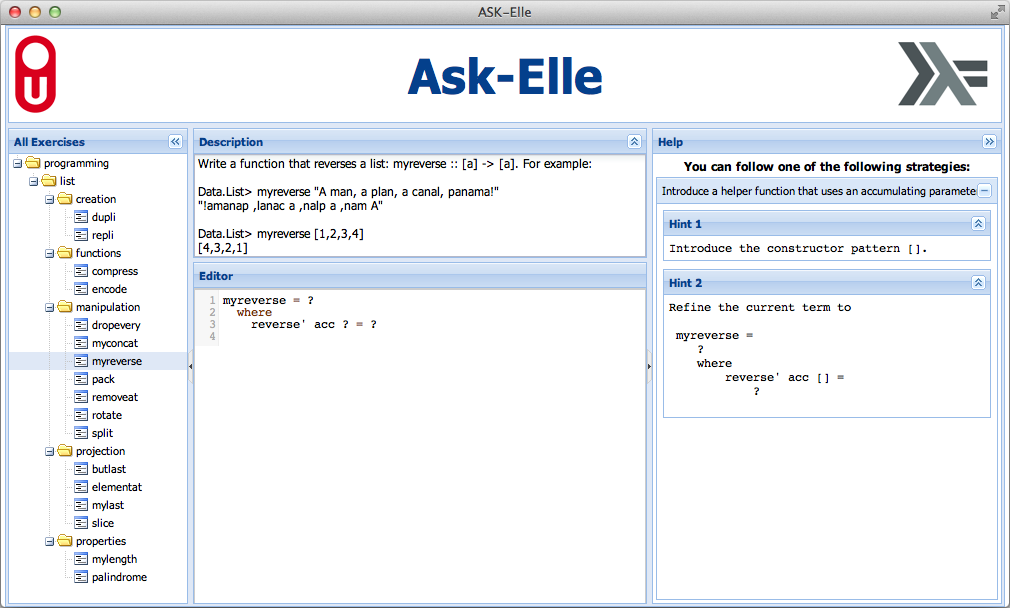
\includegraphics[scale=0.29]{fptutor.png}
\end{center}

}

\frame{\frametitle{Behind the scenes of Ask-Elle}

\begin{itemize}
	\item To define an exercise, a teacher provides \emph{model solutions}.
	\item Using \emph{strategies}, Ask-Elle compares a student's code against these model solutions
	\item If a student's code can be reduced to a model solution, Ask-Elle can provide detailed feedback and hints
	\item What happens when the student \textit{doesn't} follow a model solution?
\end{itemize}

}

\begin{frame}[fragile]
\frametitle{A gap in detailed feedback}

No model solution fits the student's solution? QuickCheck!

\begin{verbatim}
"Wrong solution: 
 range 4 6 provides a counterexample."
\end{verbatim}

Can we provide richer feedback and offer a more precise location of the programming error?

\end{frame}

\begin{frame}[fragile]
\frametitle{A gap in detailed feedback}

No model solution fits the student's solution? QuickCheck!

\begin{verbatim}
"Wrong solution: 
 range 4 6 provides a counterexample."
\end{verbatim}

Can we provide richer feedback and offer a more precise location of the programming error? \emph{Yes, with contracts!}

\end{frame}

\section{Contracts}

\frame{\frametitle{What's a contract?}

Just like its real-world counterpart, a programming contract stipulates \emph{prerequisites} and \emph{guarantees} between two parties: 
\begin{itemize}
	\item The function being called (\emph{the callee})
	\item The function receiving the result (\emph{the caller})
\end{itemize}

Simple example: the function must only accept natural numbers (\emph{a prerequisite}) and will always return natural numbers (\emph{a guarantee}).

And just like in real life, these contracts can be \emph{violated}.

}

\frame{\frametitle{Contract violations and blame assignment}

When a \emph{contract violation} occurs, blame must be assigned:
\begin{itemize}
	\item Prerequisite violation $\rightarrow$ blame is on the \emph{caller}.
	\item Guarantee violation $\rightarrow$ blame is on the \emph{callee}.
\end{itemize}

Adding contracts to your code:
\begin{itemize}
 	\item Aids in debugging 
 	\item Provides automated runtime enforcement of constraints and invariants
\end{itemize}

We use the \texttt{typed-contracts} contract library by Hinze et al.

}

\subsection{The \texttt{typed-contracts} library}

\begin{frame}[fragile]
\frametitle{Constructing a contract}

\texttt{typed-contracts} uses a GADT:

\begin{lstlisting}[mathescape]
data Contract a where
   Prop      :: (a $\rightarrow$ Bool) $\rightarrow$ Contract a
   Function  :: Contract a $\rightarrow$ (a $\rightarrow$ Contract b) $\rightarrow$ Contract (a $\rightarrowtriangle$ b)
   Pair      :: Contract a $\rightarrow$ (a $\rightarrow$ Contract b) $\rightarrow$ Contract (a, b)
   List      :: Contract a $\rightarrow$ Contract [a]
   Functor   :: Functor f $\Rightarrow$ Contract a $\rightarrow$ Contract (f a)
   Bifunctor :: Bifunctor f $\Rightarrow$ Contract a $\rightarrow$ Contract b $\rightarrow$ Contract (f a b)
   And       :: Contract a $\rightarrow$ Contract a $\rightarrow$ Contract a
\end{lstlisting}

\end{frame}

\begin{frame}[fragile]
\frametitle{Constructing a contract - \texttt{Prop} constructor}

\begin{lstlisting}[mathescape]
Prop :: (a $\rightarrow$ Bool) $\rightarrow$ Contract a
\end{lstlisting}

\begin{itemize}
	\item Lift a function to a contract
	\item Defines a constraint or property on a type
\end{itemize}

\end{frame}

\begin{frame}[fragile]
\frametitle{Constructing a contract - \texttt{Function} constructor}

\begin{lstlisting}[mathescape]
Function :: Contract a $\rightarrow$ (a $\rightarrow$ Contract b) $\rightarrow$ Contract (a $\rightarrowtriangle$ b)
\end{lstlisting}

\begin{itemize}
	\item Defines a dependent function contract
	\item Note the $\rightarrowtriangle$
\end{itemize}

\end{frame}

\begin{frame}[fragile]
\frametitle{Constructing a contract - \texttt{Pair} constructor}

\begin{lstlisting}[mathescape]
Pair :: Contract a $\rightarrow$ (a $\rightarrow$ Contract b) $\rightarrow$ Contract (a, b)
\end{lstlisting}

\begin{itemize}
	\item Defines a dependent pair
	\item Not used in this presentation
\end{itemize}

\end{frame}

\begin{frame}[fragile]
\frametitle{Constructing a contract - \texttt{List} constructor}

\begin{lstlisting}[mathescape]
List :: Contract a $\rightarrow$ Contract [a]
\end{lstlisting}

\begin{itemize}
	\item Lifts contracts to the list level
\end{itemize}

\end{frame}

\begin{frame}[fragile]
\frametitle{Constructing a contract - \texttt{Functor} constructor}

\begin{lstlisting}[mathescape]
Functor :: Functor f $\Rightarrow$ Contract a $\rightarrow$ Contract (f a)
\end{lstlisting}

\begin{itemize}
	\item A container type that can house types of kind $* \rightarrow *$
	\item Examples: \texttt{Maybe}, \texttt{Just}
\end{itemize}

\end{frame}

\begin{frame}[fragile]
\frametitle{Constructing a contract - \texttt{Bifunctor} constructor}

\begin{lstlisting}[mathescape]
Bifunctor :: Bifunctor f $\Rightarrow$ Contract a $\rightarrow$ Contract b $\rightarrow$ Contract (f a b)
\end{lstlisting}

\begin{itemize}
	\item A container type that can house types of kind $* \rightarrow * \rightarrow *$
	\item Examples: \texttt{Either}, 2-tuple
\end{itemize}

\end{frame}

\begin{frame}[fragile]
\frametitle{Constructing a contract - \texttt{And} constructor}

\begin{lstlisting}[mathescape]
And :: Contract a $\rightarrow$ Contract a $\rightarrow$ Contract a
\end{lstlisting}

\begin{itemize}
	\item Chains contracts together
	\item All contracts are asserted when a value is provided
\end{itemize}

\end{frame}

\begin{frame}[fragile]
\frametitle{Some notation for contracts}

\begin{lstlisting}[mathescape]
c$_1$ $\rightarrowtriangle$ c$_2$		= Function c$_1$ (const c$_2$)
(&)		= And
c$_1$ $\functor$ c$_2$		= c$_1$ & Functor c$_2$
c$_1$ $\bifunctor$ (c$_2$,c$_2$)	= c$_1$ & Bifunctor c$_2$ c$_3$
\end{lstlisting}

\begin{itemize}
	\item \texttt{c$_1$ $\rightarrowtriangle$ c$_2$} defines a non-dependent function contract
	\item \texttt{$\functor$} and \texttt{$\bifunctor$} use \texttt{c$_1$} as a contract that must hold on the container in its entirety: an \emph{outer contract}.
	\item Example: an ordered list
\end{itemize}

\end{frame}

\begin{frame}[fragile]
\frametitle{Constructing a contract: examples}

Fundamental contracts:

\begin{lstlisting}[mathescape]
true, false :: Contract a
true  = Prop ($\lambda$_ $\rightarrow$ True)
false = Prop ($\lambda$_ $\rightarrow$ False)
\end{lstlisting}

A contract that only allows natural numbers:

\begin{lstlisting}[mathescape]
nat :: Contract Int
nat = Prop ($\lambda$i $\rightarrow$ i $\geq$ 0)
\end{lstlisting}

\end{frame}

\begin{frame}[fragile]
\frametitle{Asserting contracts}

To attach a contract to a function, we use \texttt{assert}:

\begin{lstlisting}[mathescape]
assert :: String $\rightarrow$ Contract a $\rightarrow$ a $\rightarrow$ a
\end{lstlisting}

\texttt{assert} acts as a \emph{partial identity} function: in the case of a contract violation, an exception is thrown. Otherwise, it acts as identity.

\end{frame}

\begin{frame}[fragile]
\frametitle{Asserting contracts: an example}

\begin{lstlisting}[mathescape]
assert :: String $\rightarrow$ Contract a $\rightarrow$ a $\rightarrow$ a
\end{lstlisting}

\begin{lstlisting}[mathescape]
inc :: Int $\rightarrowtriangle$ Int
inc = assert "inc" (nat $\rightarrowtriangle$ nat) (fun ($\lambda$n $\rightarrow$ 1 + n))
\end{lstlisting}

\begin{itemize}
	\item \texttt{(nat $\rightarrowtriangle$ nat)} is of type \texttt{Contract (Int $\rightarrowtriangle$ Int)}
	\item So, \texttt{a} must be of type \texttt{(Int $\rightarrowtriangle$ Int)}
	\item \texttt{fun} lifts a single argument to the contract level:
\end{itemize}

\begin{lstlisting}[mathescape]
fun :: (a $\rightarrow$ b) $\rightarrow$ (a $\rightarrowtriangle$ b)
\end{lstlisting}

\end{frame}

\begin{frame}[fragile]
\frametitle{Asserting contracts: an example}

\begin{lstlisting}[mathescape]
inc :: Int $\rightarrowtriangle$ Int
inc = assert "inc" (nat $\rightarrowtriangle$ nat) (fun ($\lambda$n $\rightarrow$ 1 + n))
\end{lstlisting}

We use \texttt{app} to apply values to a \emph{contracted function} such as \texttt{inc}:

\begin{lstlisting}[mathescape]
app :: (a $\rightarrowtriangle$ b) $\rightarrow$ Int $\rightarrow$ a $\rightarrow$ b
\end{lstlisting}

It also labels the application with a number, used in feedback:
\begin{verbatim}
> app inc 1 5
> 5
> app inc 1 (-5)
> *** Exception: contract failed: the expression 
                 labeled `1' is to blame.
\end{verbatim}

\end{frame}

\section{Contract inference}

\begin{frame}[fragile]
\frametitle{Inferring contracts?}

\begin{itemize}
	\item Jurri\"en Stutterheim describes a way to \emph{infer} contracts for the components of a function in his thesis.
	\item Developed a contract inference algorithm: Algorithm \CW
	\item Based on Algorithm \W ~by Damas and Milner
	\item Works on a small let-polymorphic lambda calculus
\end{itemize}

Three requirements for contract inference:

\begin{itemize}
	\item Infer a well-typed contract for every component of a program
	\item Inferred contracts must allow a (non-strict) subset of the values allowed by the types
	\item The most general inferred contract must never fail an assertion
\end{itemize}

\end{frame}

\begin{frame}[fragile]
\frametitle{An intermediate contract grammar}

\begin{lstlisting}[mathescape]
$c$ ::=   $\rho_{\alpha}$
    |  $true_{\alpha}$
    |  $false_{\alpha}$
    |  $c_{\alpha} \rightarrowtriangle c_{\beta}$
    |  $c_{\alpha} \functor c_{\beta}$
    |  $c_{\alpha} \bifunctor (c_{\beta}, c_{\gamma})$
    (...)
    
$\sigma$ ::=   $c$
    |  $\forall{true_{\alpha}}.\sigma$
\end{lstlisting}

\begin{itemize}
	\item Contract grammar is library-agnostic
	\item They must be translated to a contract library of choice
	\item Instead of fresh type variables, you have fresh \textit{contract} variables
\end{itemize}

\end{frame}

\begin{frame}[fragile]
\frametitle{Examples of inferred contracts}

\begin{itemize}
	\item Function: \texttt{id :: a $\rightarrow$ a}
	\item Contract: \texttt{$true_1$ $\rightarrowtriangle$ $true_1$}
\end{itemize}

\begin{itemize}
	\item Function: \texttt{const :: a $\rightarrow$ b $\rightarrow$ a}
	\item Contract: \texttt{$true_1$ $\rightarrowtriangle$ $true_2$ $\rightarrowtriangle$ $true_1$}
\end{itemize}

\begin{itemize}
	\item Function: \texttt{map :: (a $\rightarrow$ b) $\rightarrow$ [a] $\rightarrow$ [b]}
	\item Contract: \texttt{($true_1$ $\rightarrowtriangle$ $true_2$) $\rightarrowtriangle$ ($list_1$ $\functor$ $true_1$) $\rightarrowtriangle$ ($list_2$ $\functor$ $true_2$)}
\end{itemize}

\end{frame}

\begin{frame}[fragile]
\frametitle{Stutterheim's goal: superior feedback in Ask-Elle}

\begin{itemize}
	\item If a student's code does not follow a model solution, the only feedback possible is a QuickCheck counterexample
	\item Stutterheim wanted to express the QuickCheck properties as a contract for the main function
	\item Then use contract inference to infer contracts for the rest of the code
	\item Generate code that annotates all function applications with contract assertations
	\item Finally, apply the counterexample to the annotated code
	\item A contract violation occurs and offers a more precise location for the programming error
\end{itemize}

\end{frame}

\section{Expanding on Stutterheim's work}

\begin{frame}[fragile]
\frametitle{Limitations present in Stutterheim's system}

We address:
\begin{itemize}
	\item A system for code generation is left implicit
	\item Substitutions generated by Algorithm \CW ~are placed in a global set, which may result in generating an inferred contract that causes a violation during assertion
\end{itemize}

We do \textit{not} address:

\begin{itemize}
	\item Inability of Algorithm \CW ~to handle dependent contracts
	\item Lack of constant expression contracts
	\item Full integration with the Ask-Elle programming tutor
\end{itemize}

\end{frame}

\begin{frame}[fragile]
\frametitle{Our contributions}

\begin{itemize}
	\item We extend the contract inference algorithm to the Ask-Elle syntax, based on Helium, producing Algorithm \CHW
	\item Before performing contract inference, we perform AST transformations to simplify contract inference
	\item We generate \textit{initial contracts} that simplify contract inference even further, especially in the case of mutually recursive functions
	\item Substitutions are divided into two lists: global and local, avoiding the aforementioned contract violation problem
	\item We provide a system to generate code for the \textit{typed-contracts} library
\end{itemize}

\end{frame}

\subsection{Framework overview}

\begin{frame}
\frametitle{Framework overview - 1 / 2}

\begin{center}
\includegraphics[scale=0.4]{systemoverview.pdf}
\end{center}

\end{frame}

\begin{frame}
\frametitle{Framework overview - 2 / 2}

\begin{center}
\includegraphics[scale=0.4,page=2]{systemoverview.pdf}
\end{center}

\end{frame}

\subsection{AST transformations}

\begin{frame}[fragile]
\frametitle{AST transformations - Capture lambdas}

\begin{itemize}
	\item Anonymous functions cannot be contracted: need a name
	\item Solution: bind all lambda functions to unique identifiers
	\item Referential transparency allows this
\end{itemize}

\begin{lstlisting}[mathescape]
f = $\lambda$x $\rightarrow$ x
\end{lstlisting}

is transformed into

\begin{lstlisting}[mathescape]
f = __lam0                   
 where                    
  __lam0 = $\lambda$x $\rightarrow$ x
\end{lstlisting}

\end{frame}

\begin{frame}[fragile]
\frametitle{AST transformations - Rewrite point-free functions}

\begin{itemize}
	\item \texttt{typed-contracts} does not support asserting partially applied functions
	\item all function arguments are made available on the LHS and applied to the RHS
	\item $\eta$-abstraction
\end{itemize}

\begin{lstlisting}[mathescape]
f = __lam0                   
 where                    
  __lam0 = $\lambda$x $\rightarrow$ x
\end{lstlisting}

is now transformed into

\begin{lstlisting}[mathescape]
f __a0 = (__lam0) __a0                
 where                    
  __lam0 __a0 = ($\lambda$x $\rightarrow$ x) __a0
\end{lstlisting}

\end{frame}

\begin{frame}[fragile]
\frametitle{AST transformations - Rewrite infix function applications}

\begin{itemize}
	\item Convert infix function applications to regular ones
	\item Prevent duplicate code for contract inference and code generation
	\item Removal of syntactic sugar
\end{itemize}

\end{frame}

\begin{frame}[fragile]
\frametitle{AST transformations - Expand function applications}

\begin{itemize}
	\item Split up function applications with multiple arguments into nested function applications
	\item Keeps the contract inference algorithm simple
\end{itemize}

\begin{lstlisting}
f g x y z = g x y z
\end{lstlisting}

is transformed into

\begin{lstlisting}
f g x y z = ((g x) y) z
\end{lstlisting}

\end{frame}

\begin{frame}[fragile]
\frametitle{AST transformations - Expand lambda arguments}

\begin{itemize}
	\item Split up lambdas with multiple arguments into nested ones
	\item Again, keeps the contract inference algorithm simple
\end{itemize}

\begin{lstlisting}[mathescape]
f = $\lambda$g x y z $\rightarrow$ g x y z
\end{lstlisting}

is transformed into

\begin{lstlisting}[mathescape]
f = $\lambda$g $\rightarrow$ ($\lambda$x $\rightarrow$ ($\lambda$y $\rightarrow$ ($\lambda$z $\rightarrow$ g x y z)))
\end{lstlisting}

\end{frame}

\begin{frame}
\frametitle{Framework overview - Recap}

\begin{center}
\includegraphics[scale=0.4,page=2]{systemoverview.pdf}
\end{center}

\end{frame}

\subsection{Type source}

\begin{frame}
\frametitle{What is a type source?}

\begin{itemize}
	\item A type source $\Xi$ is a data structure that may hold information about the type of a node in an AST
	\item A node can query the type source for its type with $\Xi( x )$
	\item Types are available for the following AST nodes: \texttt{Expr}, \texttt{GuardedExpr}, \texttt{Pat}, \texttt{Alt}, \texttt{FunBind} and \texttt{Rhs} 
	\item Type information is needed for some AST transformations
	\item Also useful for generating \emph{initial contracts}
\end{itemize}

\end{frame}

\begin{frame}
\frametitle{Initial contracts}

\begin{itemize}
	\item Used to simplify contract inference and code generation
	\item Captures relations between (mutually recursive) functions
\end{itemize}

Definition:
\begin{itemize}
	\item \emph{Generalized} version of the \emph{most specific} contract for that identifier
	\item Asserting contract is equal to identity
\end{itemize}

\end{frame}

\begin{frame}
\frametitle{Most-specific contracts}

Stutterheim posits a conjecture:

\begin{itemize}
	\item Any inferred contract in algorithm \CW ~is also the \emph{most specific}
	\item Contracts are represented as sets of values they allow
	\item Contract inferred for an expression $e$ is a subset of any other contract that is valid (=acts as identity) for $e$
\end{itemize}

\end{frame}

\begin{frame}
\frametitle{Generalized most-specific contracts}

A \emph{generalized} most-specific contract:

\begin{itemize}
	\item Every contract variable maps to a $true_i$ contract (so no concrete contracts like \texttt{nat})
	\item Relations present in an identifier or expression's type are also present in its contract
	\item We call them \emph{initial} contracts because they seed the contract environment of Algorithm \CHW
\end{itemize}

\end{frame}

\begin{frame}[fragile]
\frametitle{Generalized most-specific contracts - Examples}

Initial contracts for \texttt{id} and \texttt{map}:

\begin{lstlisting}[mathescape]
ctrt_id = c$_0$ $\rightarrowtriangle$ c$_0$
ctrt_map = (c$_1$ $\rightarrowtriangle$ c$_2$) $\rightarrowtriangle$ (c$_3$ $\functor$ c$_1$) $\rightarrowtriangle$ (c$_4$ $\functor$ c$_2$)
\end{lstlisting}

\textbf{Not} initial contracts:

\begin{lstlisting}[mathescape]
ctrt_id = c$_0$ $\rightarrowtriangle$ c$_1$
ctrt_map = (c$_1$ $\rightarrowtriangle$ c$_2$) $\rightarrowtriangle$ (c$_3$ $\functor$ c$_4$) $\rightarrowtriangle$ (c$_5$ $\functor$ c$_6$)
\end{lstlisting}

Why?
\begin{itemize}
	\item \texttt{id}: relation between input and output is missing
	\item \texttt{map}: relation between function, list input and result missing
\end{itemize}

\end{frame}

\subsection{Contract inference}

\begin{frame}[fragile]
\frametitle{Algorithm \CHW}

\begin{itemize}
	\item Based on Algorithm \CW (so also on Algorithm \W)
	\item Works on Ask-Elle syntax
	\item Intermediate contract grammar is trimmed: $literal_i$
	\item Contract variables are implicitly universally quantified
	\item Definition of contract environment $\Gamma$ is the same
	\item Use of type source $\Xi$ to seed $\Gamma$
	\item Requirements remain the same (well-typed, subset of type inhabitants, inferred = identity)
\end{itemize}

\end{frame}

\begin{frame}[fragile]
\frametitle{Relation between $\Gamma$ and $\Xi$}

\begin{itemize}
	\item In type inference, $\Gamma$ is updated with fresh type variables during inference
	\item These variables are later unified to infer the final type
	\item We need to infer contracts
	\item By taking initial contracts as starting point, we can focus on the inference uniquely required by contracts:
\end{itemize}

\begin{lstlisting}[mathescape]
ctrt_map = (c$_1$ $\rightarrowtriangle$ c$_2$) $\rightarrowtriangle$ (c$_3$ $\functor$ c$_1$) $\rightarrowtriangle$ (c$_4$ $\functor$ c$_2$)
\end{lstlisting}

\begin{itemize}
	\item Perhaps $c_3$ and $c_4$ are the same?
	\item Cannot derive this from the type, need inference
\end{itemize}

\end{frame}

\begin{frame}[fragile]
\frametitle{$\Xi$ does the heavy lifting}

\begin{itemize}
	\item Seed $\Gamma$ with contracts for patterns and function identifiers
	\item When new identifiers come into scope, these are added as well, shadowing previous ones
	\item Described in seeding rules
\end{itemize}

\end{frame}

\begin{frame}
\frametitle{Framework overview - Recap}

\begin{center}
\includegraphics[scale=0.4,page=2]{systemoverview.pdf}
\end{center}

\end{frame}

\subsection{Code generation}

\begin{frame}[fragile]
\frametitle{A code generation system}

\begin{itemize}
	\item Library-agnostic code generation system
	\item We can generate code for the \texttt{typed-contracts} library
	\item For each function \texttt{X}, we generate three new functions:
	\begin{itemize}
	\item \texttt{\underline{\hspace{1.5em}}final\_X}
	\item \texttt{\underline{\hspace{1.5em}}app\_X}
	\item \texttt{\underline{\hspace{1.5em}}contracted\_X}
	\end{itemize}
	\item We will look at an example of each
\end{itemize}

\end{frame}

\begin{frame}[fragile]
\frametitle{\texttt{\underline{\hspace{1.5em}}final\_X}}

\begin{itemize}
	\item Transformed copy of the original function definition
	\item Every function application is replaced by its contracted equivalent, the \texttt{\underline{\hspace{1.5em}}app\_X} template
	\item Adds position information from code for richer feedback
	\item Entry point for all other generated functions
\end{itemize}

\end{frame}

\begin{frame}[fragile]
\frametitle{\texttt{\underline{\hspace{1.5em}}final\_X} - Example}

\begin{lstlisting}[mathescape]
f x = g x
g x = [x]
\end{lstlisting}

Generated code for \texttt{f x = g x}:

\begin{lstlisting}[mathescape]
__final_f :: a $\rightarrow$ [a]
__final_f x = __app_g $ctrt$ $posg$ ($posx$,x)
\end{lstlisting}

Placeholders:
\begin{itemize}
	\item $ctrt$: contract used to assert original function (\texttt{g}, in our case)
	\item $posg$: Tuple of line and column position of application of \texttt{g}
	\item $posx$: Tuple of line and column position of  \texttt{x}
\end{itemize}

\end{frame}

\begin{frame}[fragile]
\frametitle{\texttt{\underline{\hspace{1.5em}}app\_X}}

\begin{itemize}
	\item Wraps arguments with a variation of \texttt{app} named \texttt{appParam}
	\item Passes them to the \texttt{\underline{\hspace{1.5em}}contracted\_X} template
	\item A fixed template with placeholders that are filled in:
\end{itemize}

\begin{lstlisting}[mathescape]
__app_X ctrt posinfo $(argument$ $patterns)$ = $(applied$ $arguments)$
\end{lstlisting}

Placeholders:
\begin{itemize}
	\item $(argument$ $patterns)$: for each pattern \texttt{p} of function \texttt{X}, make a tuple \texttt{(posp,p)}
	\item $(applied$ $arguments)$: wrap arguments with \texttt{appParam} and pass them to \texttt{\underline{\hspace{1.5em}}contracted\_X} template
\end{itemize}

\end{frame}

\begin{frame}[fragile]
\frametitle{\texttt{\underline{\hspace{1.5em}}app\_X} - Example}

Generated code for function definition \texttt{f x = g x}:

\begin{lstlisting}[mathescape]
type LC = Maybe (Int,Int)
__app_f :: Contract (a $\rightarrowtriangle$ [a]) $\rightarrow$ LC $\rightarrow$ (LC,a) $\rightarrow$ [a]
__app_f ctrt posinfo (posx,x) =
 appParam (__contracted_f ctrt posinfo) (show x ++ generatePositionData posx) x
\end{lstlisting}

\texttt{app} takes an integer as a position label to use in feedback, \texttt{appParam} takes a string:

\begin{lstlisting}[mathescape]
app :: (a $\rightarrowtriangle$ b) $\rightarrow$ Int $\rightarrow$ a $\rightarrow$ b
appParam :: (a $\rightarrowtriangle$ b) $\rightarrow$ String $\rightarrow$ a $\rightarrow$ b
\end{lstlisting}

\end{frame}

\begin{frame}[fragile]
\frametitle{\texttt{\underline{\hspace{1.5em}}contracted\_X}}

\begin{itemize}
	\item Constructs an assertion with the contract provided
	\item A fixed template with placeholders that are filled in:
\end{itemize}

\begin{lstlisting}[mathescape]
__contracted_X ctrt posinfo = assertPos $(function$ $info)$ 
 (generatePositionData posinfo) ctrt funs
  where funs = $(contracted$ $function$ $definition)$
\end{lstlisting}

Placeholders:
\begin{itemize}
	\item \textit{function info}: String identifying the function responsible for the violation, for feedback purposes
	\item \textit{contracted function definition}: Using \texttt{fun}, the function is lifted to a contracted version
\end{itemize}

\end{frame}

\begin{frame}[fragile]
\frametitle{\texttt{\underline{\hspace{1.5em}}contracted\_X} - Example}

Generated code for function definition \texttt{f x = g x}:
\begin{lstlisting}[mathescape]
__contracted_f :: Contract (a $\rightarrowtriangle$ b) $\rightarrow$ LC $\rightarrow$ (a $\rightarrowtriangle$ a)
__contracted_f ctrt posinfo = assertPos "f" 
 (generatePositionData posinfo) ctrt funs
  where funs = fun ($\lambda$x $\rightarrow$ __final_f x)
\end{lstlisting}

\begin{itemize}
	\item \texttt{assertPos} takes position information for more precise feedback
	\item Remember that \texttt{\underline{\hspace{1.5em}}final\_f} calls \texttt{\underline{\hspace{1.5em}}app\_g}
	\item For recursive functions: cycle of \texttt{\underline{\hspace{1.5em}}final\_X} $\rightarrow$ \texttt{\underline{\hspace{1.5em}}app\_X} $\rightarrow$ \texttt{\underline{\hspace{1.5em}}contracted\_X} $\rightarrow$ \texttt{\underline{\hspace{1.5em}}final\_X} until base case is reached
\end{itemize}

\end{frame}

\begin{frame}
\frametitle{Framework overview - Recap}

\begin{center}
\includegraphics[scale=0.4,page=2]{systemoverview.pdf}
\end{center}

\end{frame}

\subsection{Generation of final contracts}

\begin{frame}
\frametitle{Contract translation and substitution application}

\begin{itemize}
	\item Remember, inferred contracts are written in an intermediate contract language
	\item \emph{Translation} to a target library required
	\item First, an example: \texttt{typed-contracts}
	\item Then: How substitutions are applied
	\item Translation occurs after substitutions
\end{itemize}

\end{frame}

\begin{frame}
\frametitle{Translation to \texttt{typed-contracts}}

Intermediate contract language is inspired by \textit{typed-contracts}' notation, so translation is easy:

\begin{itemize}
	\item $true_i$ $\rightarrow$ \texttt{true}
	\item $false_i$ $\rightarrow$ \texttt{false}
	\item ($\rightarrowtriangle$), ($\functor$) and ($\bifunctor$) translate directly
	\item $literal_i$ $\rightarrow$ \texttt{true} (future work)
	\item $\rho_{\alpha}$: $\alpha$ is just a string that is printed during code generation
\end{itemize}

\end{frame}

\begin{frame}
\frametitle{Substitutions in Stutterheim's proof-of-concept}

\begin{itemize}
	\item All substitutions are placed in a global set
	\item In some circumstances, may violate the "inferred = identity" requirement
\end{itemize}

\end{frame}

\begin{frame}[fragile]
\frametitle{The counterexample - 1 / 3}

\begin{lstlisting}
g x = [x]
z = (g 'a', g 5)
\end{lstlisting}

\begin{lstlisting}[mathescape]
$\Gamma$(z) = true$_0$ $\bifunctor$ (true$_1$ $\functor$ isChar, true$_2$ $\functor$ isNum)
\end{lstlisting}

During inference: 

\begin{lstlisting}[mathescape]
$\Gamma$(x) 	  = true$_4$
$\Gamma$(g) 	  = true$_4$ $\rightarrowtriangle$ (true$_3$ $\functor$ true$_4$)
$\Gamma$('a') = true$_5$
$\Gamma$(5) 	  = true$_6$
\end{lstlisting}

\begin{lstlisting}[mathescape]
-- Unification of first argument of g with 'a'
unify (true$_4$) (true$_5$)

-- Unification of first argument of g with 5
unify (true$_4$) (true$_6$)
\end{lstlisting}

\end{frame}

\begin{frame}[fragile]
\frametitle{The counterexample - 2 / 3}

\begin{lstlisting}[mathescape]
-- Unification of first argument of g with 'a'
unify (true$_4$) (true$_5$)

-- Unification of first argument of g with 5
unify (true$_4$) (true$_6$)
\end{lstlisting}

Resulting substitutions: \texttt{true$_4$ $\mapsto$ true$_5$}, \texttt{true$_4$ $\mapsto$ true$_6$}

Apply substitutions to RHS of \texttt{z}, which has contract \texttt{(true$_7$ $\bifunctor$ (true$_3$ $\functor$ true$_4$, true$_3$ $\functor$ true$_4$))}:

\begin{itemize}
	\item left-to-right: \texttt{(true$_7$ $\bifunctor$ (true$_3$ $\functor$ true\emph{$_5$}, true$_3$ $\functor$ true\emph{$_5$}))}
	\item right-to-left: \texttt{(true$_7$ $\bifunctor$ (true$_3$ $\functor$ true\emph{$_6$}, true$_3$ $\functor$ true\emph{$_6$}))}
\end{itemize}

\end{frame}

\begin{frame}[fragile]
\frametitle{The counterexample - 3 / 3}

Unify with contract of \texttt{z}:

\begin{lstlisting}[mathescape]
unify (true$_0$ $\bifunctor$ (true$_1$ $\functor$ isChar, true$_2$ $\functor$ isNum))
      (true$_7$ $\bifunctor$ (true$_3$ $\functor$ true$_5$, true$_3$ $\functor$ true$_5$))
\end{lstlisting}

Relevant substitutions: \texttt{true$_5$ $\mapsto$ isChar}, \texttt{true$_5$ $\mapsto$ isNum}

\begin{lstlisting}[mathescape]
unify (true$_0$ $\bifunctor$ (true$_1$ $\functor$ isChar, true$_2$ $\functor$ isNum))
      (true$_7$ $\bifunctor$ (true$_3$ $\functor$ true$_6$, true$_3$ $\functor$ true$_6$))
\end{lstlisting}

Relevant substitutions: \texttt{true$_6$ $\mapsto$ isChar}, \texttt{true$_6$ $\mapsto$ isNum}

Applying these substitutions always results in an incorrect contract:
\begin{itemize}
\item left-to-right: contract of \texttt{g 5} is \texttt{(true$_1$ $\functor$ isChar)}
\item right-to-left: contract of \texttt{g 'a'} is \texttt{(true$_1$ $\functor$ isNum)}
\end{itemize}

\end{frame}

\begin{frame}[fragile]
\frametitle{Solution: Global and local substitution lists}

\begin{itemize}
	\item Contract variables are given a flavour of global or local
	\item $true_i$ contracts are global
	\item Concrete contracts (like \texttt{nat}) are local
	\item Whenever unification takes place, split substitutions into two groups
	\item Global group: all substitutions from global $\rightarrow$ global
	\item Local group: all substitutions from global $\rightarrow$ local and local $\rightarrow$ local
	\item Global group is added to global list (up the AST)
	\item Local group is kept in the node where unification took place, also passed down to children (down the AST)
\end{itemize}

\end{frame}

\begin{frame}[fragile]
\frametitle{A snare in the plan!}

\begin{itemize}
	\item First, apply globals, then update locals, then apply locals
	\item Applying these substitutions statically presents a problem:
\end{itemize}

\begin{lstlisting}
f x = g x
g x = [x]
z = (f 'a', f 5)
\end{lstlisting}

\begin{lstlisting}[mathescape]
__final_f x = __app_g (c1 $\rightarrowtriangle$ (c2 $\functor$ c1)) x
 where c1 = true
       c2 = true
__final_g x = [x]
__final_z = (__app_f (isChar $\rightarrowtriangle$ (true $\functor$ isChar)) 'a', __app_f (isNum $\rightarrowtriangle$ (true $\functor$ isNum)) 5)
\end{lstlisting}

\begin{itemize}
	\item The local substitutions that made the contract passed to \texttt{\_\_app\_f} more specific, are not utilized by \texttt{\_\_app\_g}
	\item Solution: Pass around and apply local substitutions at runtime
\end{itemize}

\end{frame}

\begin{frame}
\frametitle{An even bigger snare in the plan!}

\begin{itemize}
	\item Substitutions only work on intermediate contract language
	\item But generated code expects contracts of targeted library!
	\item Runtime translation of intermediate contract language and target library is required
	\item \texttt{typed-contracts} contract is defined as a GADT with a phantom type for type-level representation of the contract
	\item Intermediate contract language is a UUAGC-generated regular data type
	\item Need a way to recover the extra type information
	\item Explored several avenues, left as future work
\end{itemize}

\end{frame}

\section{Results}

\begin{frame}[fragile]
\frametitle{Ask-Elle's feedback versus our framework's feedback}

\begin{itemize}
	\item The feedback we generate is at least as informative as that of Ask-Elle
	\item Can't do much if code does not contain any function applications:

\begin{lstlisting}
myreverse [] = []
myreverse [x,y] = [x,y]
myreverse xs = ?	
\end{lstlisting}
	
	\item Automatically translating QuickCheck properties to contracts is often suboptimal, if doable at all:
	
\begin{lstlisting}[mathescape]
prop_Main = $\lambda$xs n $\rightarrow$ n > 0 ==> concatMap (replicate n) xs == repli xs n
\end{lstlisting}

	\item Custom contracts offer better feedback capabilities
\end{itemize}

\end{frame}

\begin{frame}[fragile]
\frametitle{Ask-Elle's feedback versus our framework's feedback - Custom contracts}

\begin{lstlisting}[mathescape,numbers=left]
insert z zs = case zs of
                [] $\rightarrow$ [z]
                (z':zs') $\rightarrow$ in case z <= z' of
                               True $\rightarrow$ z' : z : zs'
                               False $\rightarrow$ z' : insert z zs'
foldr f b xs = case xs of
                [] $\rightarrow$ b
                (y:ys) $\rightarrow$ f y (foldr f b ys)
                
isort us = foldr insert [] us
\end{lstlisting}

The following QuickCheck property is checked, and fails:

\begin{lstlisting}[mathescape]
prop_Main = $\lambda$xs $\rightarrow$ whenFail (putStrLn "The list elements must be in ascending order.") (isOrdered xs)
\end{lstlisting}

QuickCheck reports a counterexample of \texttt{[0,1]}

\end{frame}

\begin{frame}[fragile]
\frametitle{Ask-Elle's feedback versus our framework's feedback - Custom contracts}

Our custom contract:

\begin{lstlisting}[mathescape]
isort_ctrt = (true $\functor$ true) $\rightarrowtail$ (ord $\functor$ true)
 where ord = PropInfo ($\lambda$x $\rightarrow$ isOrdered x) ($\lambda$p $\rightarrow$ mkErrorMsg p "the list elements must be in ascending order.") 
\end{lstlisting}

Code is generated, and we apply \texttt{\underline{\hspace{1.5em}}final\_isort} to \texttt{[0,1]}...

\end{frame}

\begin{frame}[fragile]
\frametitle{Ask-Elle's feedback versus our framework's feedback - Custom contracts}

\begin{lstlisting}[mathescape,numbers=left]
insert z zs = case zs of
                [] $\rightarrow$ [z]
                (z':zs') $\rightarrow$ in case z <= z' of
                               True $\rightarrow$ z' : z : zs'
                               False $\rightarrow$ z' : insert z zs'
foldr f b xs = case xs of
                [] $\rightarrow$ b
                (y:ys) $\rightarrow$ f y (foldr f b ys)
                
isort us = foldr insert [] us
\end{lstlisting}

\begin{quote}
\textit{A part of your code, or a supplied argument to a function, does not fulfill a required property. This occurred at the application of the function 'insert' at line number 10, column number 19. The result of this function does not fulfill the following property: the list elements must be in ascending order.}
\end{quote}

\end{frame}

\begin{frame}[fragile]
\frametitle{Ask-Elle's feedback versus our framework's feedback - Custom contracts}

\begin{itemize}
	\item The issue lies with \texttt{insert}
	\item Cut down search space a little
	\item In bigger programs, search space will be cut down by a lot more
\end{itemize}

\end{frame}

\begin{frame}[fragile]
\frametitle{Ask-Elle's feedback versus our framework's feedback - Custom contracts}

Let's rectify the error (it should be \texttt{z : z' : zs'})...

\begin{lstlisting}[mathescape,numbers=left]
insert z zs = case zs of
                [] $\rightarrow$ [z]
                (z':zs') $\rightarrow$ in case z <= z' of
                               True $\rightarrow$ z' : z : zs'
                               False $\rightarrow$ z' : insert z zs'
foldr f b xs = case xs of
                [] $\rightarrow$ b
                (y:ys) $\rightarrow$ f y (foldr f b ys)
                
isort us = foldr insert [] us
\end{lstlisting}

\end{frame}

\begin{frame}[fragile]
\frametitle{Ask-Elle's feedback versus our framework's feedback - Custom contracts}

Let's rectify the error (it should be \texttt{z : z' : zs'})...

\begin{lstlisting}[mathescape,numbers=left]
insert z zs = case zs of
                [] $\rightarrow$ [z]
                (z':zs') $\rightarrow$ in case z <= z' of
                               True $\rightarrow$ z : z' : zs'
                               False $\rightarrow$ z' : insert z zs'
foldr f b xs = case xs of
                [] $\rightarrow$ b
                (y:ys) $\rightarrow$ f y (foldr f b ys)
                
isort us = foldr insert [] us
\end{lstlisting}

\end{frame}

\begin{frame}[fragile]
\frametitle{Ask-Elle's feedback versus our framework's feedback - Custom contracts}

And introduce another by changing \texttt{z <= z'} to \texttt{z' <= z}:

\begin{lstlisting}[mathescape,numbers=left]
insert z zs = case zs of
                [] $\rightarrow$ [z]
                (z':zs') $\rightarrow$ in case z <= z' of
                               True $\rightarrow$ z : z' : zs'
                               False $\rightarrow$ z' : insert z zs'
foldr f b xs = case xs of
                [] $\rightarrow$ b
                (y:ys) $\rightarrow$ f y (foldr f b ys)
                
isort us = foldr insert [] us
\end{lstlisting}

\end{frame}

\begin{frame}[fragile]
\frametitle{Ask-Elle's feedback versus our framework's feedback - Custom contracts}

And introduce another by changing \texttt{z <= z'} to \texttt{z' <= z}:

\begin{lstlisting}[mathescape,numbers=left]
insert z zs = case zs of
                [] $\rightarrow$ [z]
                (z':zs') $\rightarrow$ in case z' <= z of
                               True $\rightarrow$ z : z' : zs'
                               False $\rightarrow$ z' : insert z zs'
foldr f b xs = case xs of
                [] $\rightarrow$ b
                (y:ys) $\rightarrow$ f y (foldr f b ys)
                
isort us = foldr insert [] us
\end{lstlisting}

\end{frame}

\begin{frame}[fragile]
\frametitle{Ask-Elle's feedback versus our framework's feedback - Custom contracts}

Let's apply the counterexample again...

\begin{lstlisting}[mathescape,numbers=left]
insert z zs = case zs of
                [] $\rightarrow$ [z]
                (z':zs') $\rightarrow$ in case z' <= z of
                               True $\rightarrow$ z : z' : zs'
                               False $\rightarrow$ z' : insert z zs'
foldr f b xs = case xs of
                [] $\rightarrow$ b
                (y:ys) $\rightarrow$ f y (foldr f b ys)
                
isort us = foldr insert [] us
\end{lstlisting}

\end{frame}

\begin{frame}[fragile]
\frametitle{Ask-Elle's feedback versus our framework's feedback - Custom contracts}

\begin{lstlisting}[mathescape,numbers=left]
insert z zs = case zs of
                [] $\rightarrow$ [z]
                (z':zs') $\rightarrow$ in case z' <= z of
                               True $\rightarrow$ z : z' : zs'
                               False $\rightarrow$ z' : insert z zs'
foldr f b xs = case xs of
                [] $\rightarrow$ b
                (y:ys) $\rightarrow$ f y (foldr f b ys)
                
isort us = foldr insert [] us
\end{lstlisting}

\begin{quote}
\textit{A part of your code, or a supplied argument to a function, does not fulfill a required property. This occurred at the application of the function ':' at line number 4, column number 45. The result of this function does not fulfill the following property: the list elements must be in ascending order.}
\end{quote}

\end{frame}

\begin{frame}[fragile]
\frametitle{Ask-Elle's feedback versus our framework's feedback - Custom contracts}

\begin{itemize}
	\item Something is wrong with \texttt{z' : zs'}: one of the elements is causing the list to no longer be ordered
	\item We cannot get closer to the problem: the contract of \texttt{(<=)} is \texttt{(true $\rightarrowtriangle$ (true $\rightarrowtriangle$ true))}
	\item Still, far more detailed feedback than Ask-Elle
\end{itemize}

\end{frame}

\section{Future work}

\begin{frame}
\frametitle{Future work}

\begin{itemize}
	\item Full integration with Ask-Elle
	\begin{itemize}
		\item Capture QuickCheck counterexamples and make them available to framework
		\item Modify exercise configuration files to contain contracts
		\item Run Prelude through the framework
	\end{itemize}
	\item \textit{Decoupling} from Ask-Elle: framework is only tightly bound to Helium for the type source
	\item Initial contract generation algorithm does not support user-defined data types
	\item Runtime translation of intermediate contract language
	\item Improve algorithm for finding final contracts
	\item Add support for partially applied function arguments to higher-order functions in code generation
	\item Use paramorphisms to tackle dependent contracts
\end{itemize}

\end{frame}

\section{Conclusions}

\begin{frame}
\frametitle{Conclusions}

Main objectives:
\begin{itemize}
	\item Extend Stutterheim's contract inference algorithm to Ask-Elle syntax
	\item Construct a code generation system
\end{itemize}

Implementation:
\begin{itemize}
	\item Constructed a framework coupling contract inference and code generation
	\item Algorithm \CHW ~builds upon Algorithm \CW
	\item Library-agnostic code generation system, little code duplication required
	\item Example implementation for \texttt{typed-contracts} library
	\item Substitution problem was largely solved
\end{itemize}

\end{frame}

\section*{Questions?}

\end{document}